\chapter{Ciclo 1}
  
  Este capítulo descreve o planejamento realizado e os resultados obtidos com a execução do primeiro ciclo da pesquisa-ação.
  
  \section{Planejamento}
  
      Após a realização do diagnóstico, era necessário um esforço inicial de configuração do \textit{framework} para a 
      adequação do PHPUnit ao CodeIgniter. Além disso, era necessário estabelecer a estrutura do \textit{framework},
      sua arquitetura de funcionamento. Portanto, ficaram definidas como escopo do primeiro ciclo as seguintes atividades:
      
      \begin{itemize}
	
	\item Configurar o CodeIgniter para receber o PHPUnit;
	
	\item Estabelecer arquitetura de funcionamento do \textit{framework}.
	
      \end{itemize}
      
      
      \subsection{Planejamento da avaliação}
      
	  Como este ciclo não agregou muito valor para a atividade de testes dos desenvolvedores do SiGA,
	  embora imprescindível para o \textit{framework}, o mesmo teve uma forma de avaliação diferente
	  dos outros ciclos (não avaliado pelo questionário proposto) por não envolver diretamente os desenvolvedores e se
	  tratar de conteúdo mais técnico inerente à equipe de desenvolvimento do \textit{framework}. Visto isso, ficou proposta
	  a seguinte estrutura de avaliação para as atividades realizadas neste ciclo:
	  
	  \begin{itemize}
	  
	    \item Para a atividade de configuração do CodeIgniter para o uso do PHPUnit:
	  
		\begin{enumerate}
	      
		  \item Testar as configurações propostas em um projeto vazio do CodeIgniter versão 2.x;
		  
		  \item Testar as configurações propostas no SiGA;
		  
		\end{enumerate}
	      
	    \item Para a atividade de estabelecimento da arquitetura de funcionamento do \textit{framework}:
		
		\begin{enumerate}
	
		  \item Validar a arquitetura proposta implementando os comandos \textit{\textbf{init}} e \textit{\textbf{help}};
		      
		      \subitem Se atentar aos seguintes itens indispensáveis:
			\begin{itemize}
			  \item É fácil de se criar um novo comando?
			  \item É possível criar um comando com parâmetros diferentes?
			  \item É possível ter parâmetros opcionais nos comandos?
			  \item É possível tratar cada comando individualmente e executá-los em conjunto?
			\end{itemize}
		  
		  \item Testar o comando \textit{\textbf{init}} em um projeto vazio do CodeIgniter versão 2.x;
		  
		  \item Testar o comando \textit{\textbf{init}} no SiGA;
	
		  \item Testar o comando \textit{\textbf{help}};
		\end{enumerate}
	  
	  \end{itemize}
  
  \section{Execução do ciclo}
  
      Esta seção apresenta detalhes relacionados à execução do ciclo 1.
      
      \subsection{Arquitetura do \textit{Ignitest}}
      
	  Para o contexto proposto, onde existirão vários comandos que possuem comportamentos únicos e bem definidos que serão
	  invocados pela linha de comando, a arquitetura definida se baseia no padrão de projeto \textit{Command} \cite{gamma}
	  com a adição de classes \textit{experts} (padrão GRASP) de metadados para cada comando, como pode ser visto na
	  figura \ref{ignitest-architecture}.
	   
	  As classes filhas da classe \textit{Command} representam um comando específico do \textit{framework} que possui sua 
	  própria implementação de execução. Cada comando possui uma classe de metadados associada a ele para descrever suas
	  informações, onde essa classe deve herdar da classe \textit{Metadata}. Os comandos informados pela linha de comando (CLI)
	  são interpretados pela classe \textit{CommandChecker}, que verifica os comandos informados, cria as instâncias respectivas
	  e adiciona os comandos na fila de execução. Os comandos disponíveis no \textit{framework} devem ser registrados na classe
	  \textit{AvailableCommand} para que seja possível a classe \textit{CommandChecker} identificar os comandos informados.
	  
	  \vfill
	  \pagebreak
	  \begin{figure}[!htb]
	    \centering
	    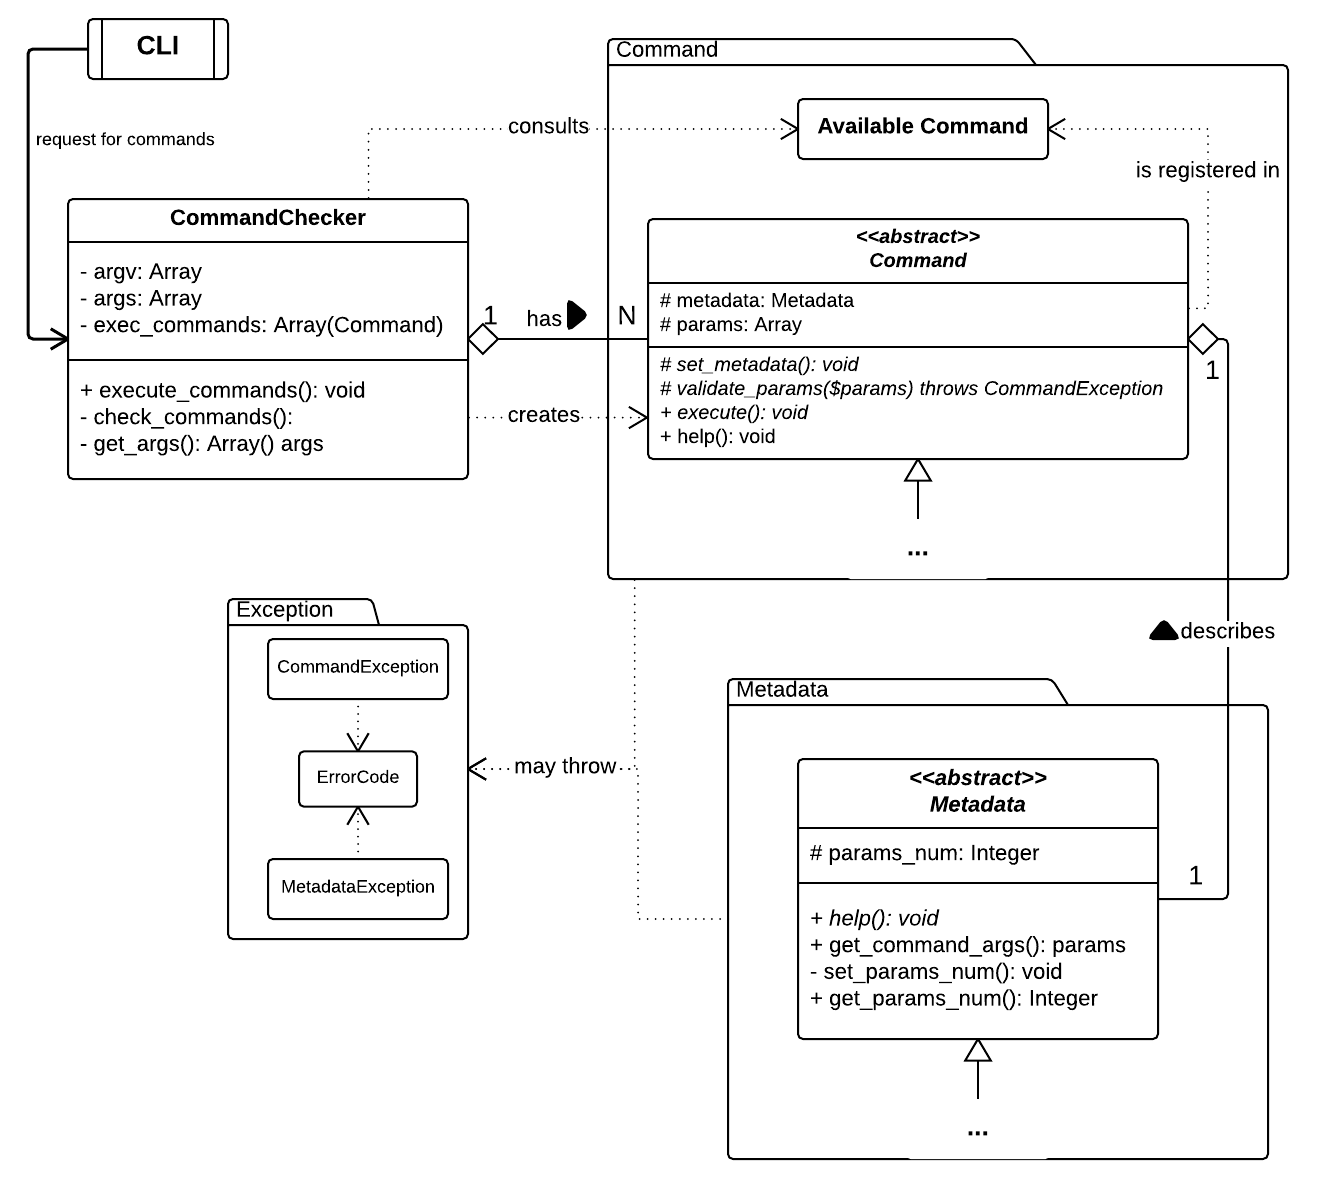
\includegraphics[scale=0.35]{figuras/ignitest-architecture.png}
	    \caption{Arquitetura do \textit{framework} proposto.}
	    \label{ignitest-architecture}
	  \end{figure}
      
      \subsection{Configurações}
	  
	  Para que o PHPUnit funcione no CodeIgniter, descobriu-se que era preciso definir um \textit{hook}\footnotemark
	  no projeto para mostrar os resultados do PHPUnit caso o ambiente fosse de teste, pois ao executar o PHPUnit nenhum
	  resultado era disponibizado na tela. Foi preciso seguir os seguintes passos para resolver esse problema:
	  \footnotetext{CodeIgniter Hooks. Disponível em \url{http://www.codeigniter.com/userguide2/general/hooks.html}. Acesso em 20/06/2016.}
	  
	  \begin{itemize}
	  
	   \item Habilitar o uso de \textit{hooks} no CodeIgniter no arquivo '\textbf{application/config/config.php}':
	      
	      \begin{verbatim}
		$config['enable_hooks'] = TRUE;
	      \end{verbatim}
	      
	   \vfill
	   \pagebreak
	   \item Criar o seguinte \textit{array} no arquivo '\textbf{application/config/hooks.php}':
	  
	      \begin{lstlisting}
		$hook['display_override'] = array(
		    'class' => 'DisplayHook',
		    'function' => 'captureOutput',
		    'filename' => 'DisplayHook.php',
		    'filepath' => 'hooks'
		);
	      \end{lstlisting}
	   
	   \item Criar a seguinte classe no diretório '\textbf{/application/hooks/}' sob o nome '\textbf{DisplayHook.php}':
	  
	  \begin{lstlisting}
	  
	      <?php
	      
	      class DisplayHook {
	          public function captureOutput() {

	              $this->CI =& get_instance();
			  
	              $output = $this->CI->output->get_output();

	              if (ENVIRONMENT != 'testing') {
	                  echo $output;
	              }
	          }
	      }
	  \end{lstlisting}
	  
	  \end{itemize}
	  
	  Além dos passos acima, são necessárias as configurações essenciais do PHPUnit, que são descritas abaixo:
	  
	  \begin{itemize}
	    \item Criar o arquivo de configuração do PHPUnit '\textbf{\textit{phpunit.xml}}' 
		  no diretório '\textbf{application/tests/}';
	    
	    \item Criar o arquivo de inicialização para os testes '\textbf{\textit{bootstrap.php}}'
		  no diretório '\textbf{application/tests/}';
	      
		\subitem Este arquivo é executado antes dos testes. Para o uso no CodeIgniter, esse arquivo deve ser
			 adaptado para conter o mesmo conteúdo do arquivo de inicialização do CodeIgniter '\textbf{index.php}', 
			 para que os recursos do CodeIgniter estejam disponíveis durante os testes.
	  \end{itemize}
	  
	  Durante a execução do ciclo, percebeu-se que era necessária bastante configuração para que o PHPUnit rodasse no
	  CodeIgniter e, portanto, parte dessa configuração, as configurações essenciais do PHPUnit, foi abstraída para
	  dentro do \textit{framework} no comando \textit{\textbf{init}}, para diminuir a carga de configuração
	  para o desenvolvedor.
  
  \section{Resultados obtidos}
    
      Este ciclo produziu os seguintes resultados:
      
      \begin{itemize}

	\item Configuração do PHPUnit ao CodeIgniter estabelecida;
	
	\item Arquitetura do \textit{framework} estabelecida;
	
	\item Comando \textit{\textbf{init}}, para automatizar parte da configuração.

      \end{itemize}

  \section{Avaliação dos resultados}
      Esta seção descreve os resultados das avaliações de configurações e arquitetura propostas, bem como pontos a serem melhorados.

      \subsection{Avaliação das configurações}
      
	  Ao tentar aplicar as configurações propostas em um novo projeto do CodeIgniter, ocorreram alguns erros referentes
	  à configuração do PHPUnit com o CodeIgniter, as quais foram sanadas da seguinte forma:
	  
	  \begin{itemize}

	    \item Configuração de protocolo URI: o protocolo em questão não pode ser automático, assim, foi necessário modificá-lo para
	    o tipo "REQUEST\_URI".
	    
	    \item Classe CI\_Utf8: era necessário carregar as configurações do CodeIgniter ao inicializar a classe.

	  \end{itemize}
	  
	  No sistema SiGA foram identificados os mesmos erros referentes às configurações.
      
      \subsection{Avaliação da arquitetura}
	  Percebeu-se que a arquitetura do \textit{framework} foi bem estrutura com o uso do padrão de projeto \textit{Command}, 
	  uma vez que facilmente é possivel criar novos comandos definindo-se uma classe para o mesmo e adicionando-o aos comandos
	  existentes.
	  
	  A criação de um comando com parâmetros diferentes foi identificada e possível graças aos metadados vinculados ao mesmo, 
	  os quais podem descrever a quantidade de parâmetros que um comando possuirá, além disso, cada metadado define como os 
	  argumentos do comando serão coletados, ou seja, caso hajam argumentos opcionais basta que os mesmos sejam tratados.
	  
	  Foi possível realizar a execução de vários comandos em conjunto, uma vez que o módulo \textit{CommandChecker} se encarrega 
	  de identificar os comandos enviados, validá-los e adicioná-los à fila de execução.
	  
	  Não ocorreram problemas ao executar os comandos \textit{init} e \textit{help} em um projeto vazio e no SiGA. 
	  
      
      \subsection{Melhorias identificadas}
	  Com todas as dificuldades encontradas durante a avaliação, percebeu-se que seria interessante embutir no comando 
	  \textit{\textbf{init}} todas as configurações realizadas manualmente, para que novos usuários não tenham tais problemas.
    

\chapter{Ciclo 2}

  Este capítulo descreve o planejamento realizado e os resultados obtidos com a execução do segundo ciclo da pesquisa-ação.
  
  \section{Planejamento}
  
      Para compor o escopo do segundo ciclo ficaram alocadas as seguintes funcionalidades, com suas respectivas características:
      
     \begin{itemize}
      \item \textbf{Criação da classe base para testes unitários;}
	\begin{itemize}
	  \item Reconhecimento da classe que está sendo testada por convenção de nomenclatura;
	\end{itemize}

      \item \textbf{Classe base para testes de integração.}
	\begin{itemize}
	  \item Reconhecimento da classe que está sendo testada por convenção de nomenclatura;
	  \item Esquema de criação e destruição do banco de testes;
	  \item Definição de dados iniciais no banco de testes;
	\end{itemize}
      \end{itemize}

  \section{Execução do ciclo}
      
      Sincronização dos banco de dados.
  
  \section{Resultados obtidos}
  
  
  \section{Avaliação dos resultados}
  
    \subsection{Melhorias identificadas}
    
\chapter{Ciclo 3...n}
  
  O tempo para a realização do trabalho não permitiu a execução de mais de um
  ciclo,embora o planjemento inicial tenha previsto mais de um ciclo. Todavia, sabe-se que o escopo dos próximos
  ciclos seria estabilizar as funcionalidades propostas do \textit{framework} com base nas melhorias identificadas
  no final de cada ciclo.
  
  A quantidade de ciclos foi estabelecida como indefinida, pois seriam executados
  ciclos até que o \textit{framework} se tornasse estável.
  